\subsection{Graph 1}\label{Graph1}

First graph database is showcasing relationships between chat join, leave, mention and respond. By that we can see what chat sessions seems to be the most active.

How data was inserted can be seen in Python code bellow.
\begin{listing}[H]
\caption{User sessions -part 1}
\begin{minted}{Python}
def create_user_sessions(data_chat_join_team_chat, 
                         data_chat_leave_team_chat, 
                         data_chat_mention_team_chat, 
                         data_chat_respond_team_chat):
    uri, user, password = get_creds(0)
    driver = GraphDatabase.driver(uri, auth=(user, password))

    create_user_query = "CREATE (:User {id: $user_id})"
    create_teamchat_session_query = 
        "CREATE (:TeamchatSession {id: $teamchat_session_id, date: $date})"
    create_chat_item_query = "CREATE (:ChatItem {id: $chat_item})"
    create_chat_relation_query = 
        "MATCH (c1), (c2) WHERE 
            c1.id = $chatid1 AND 
            c2.id = $chatid2 CREATE (c1)-[:RESPONDS_TO]->(c2)"
    create_mention_relation_query = 
        "MATCH (u), (c) WHERE 
            u.id = $user_id AND 
            c.id = $chat_item CREATE (u)-[:MENTIONS]->(c)"
    create_join_relation_query = 
        "MATCH (u), (t) WHERE 
            u.id = $user_id AND 
            t.id = $teamchat_session_id CREATE (u)-[:JOINS]->(t)"
    create_leave_relation_query = 
        "MATCH (u), (t) WHERE 
            u.id = $user_id AND 
            t.id = $teamchat_session_id CREATE (u)-[:LEAVES]->(t)"
\end{minted}
\end{listing}

\begin{listing}[H]
\caption{User sessions -part 2}
\begin{minted}{Python}
    queries = [
        (create_user_query, 
            data_chat_join_team_chat.select("user_id")
            .distinct()),
        (create_teamchat_session_query, 
            data_chat_join_team_chat
            .select("teamchat_session_id", "date")
            .distinct()),
        (create_chat_item_query, 
            data_chat_mention_team_chat
            .select("chat_item")
            .distinct()),
        (create_chat_relation_query, 
            data_chat_respond_team_chat
            .select("chatid1", "chatid2")),
        (create_mention_relation_query, 
            data_chat_mention_team_chat
            .select("user_id", "chat_item")),
        (create_join_relation_query, 
            data_chat_join_team_chat
            .select("user_id", "teamchat_session_id")),
        (create_leave_relation_query, 
            data_chat_leave_team_chat
            .select("user_id", "teamchat_session_id"))
    ]

    with driver.session() as session:
        for query, data in queries:
            for row in data.collect():
                session.run(query, **row.asDict())
\end{minted}
\end{listing}

\begin{landscape}
  \begin{figure}[H]
    \includegraphics[scale=0.047]{img/Neo4j/graph0.png}
    \centering
    \caption{Graph 1}
    \label{fig:Graph 1}
  \end{figure}
\end{landscape}

If we want to filter the nodes by the most mentioned, we can use Cypher code from bellow. This will showcase top mentioned nodes and their relations.

\begin{listing}[H]
\caption{Cypher filter 1}
\begin{minted}{Cypher}
MATCH (n)-[r]->()
WHERE TYPE(r) IN ['RESPONDS_TO', 'MENTIONS', 'JOINS', 'LEAVES']
WITH n, COUNT(*) AS mentionsCount
ORDER BY mentionsCount DESC
LIMIT 10
MATCH (n)-[r]->(m)
RETURN n, r, m
\end{minted}
\end{listing}

\begin{landscape}
  \begin{figure}[H]
    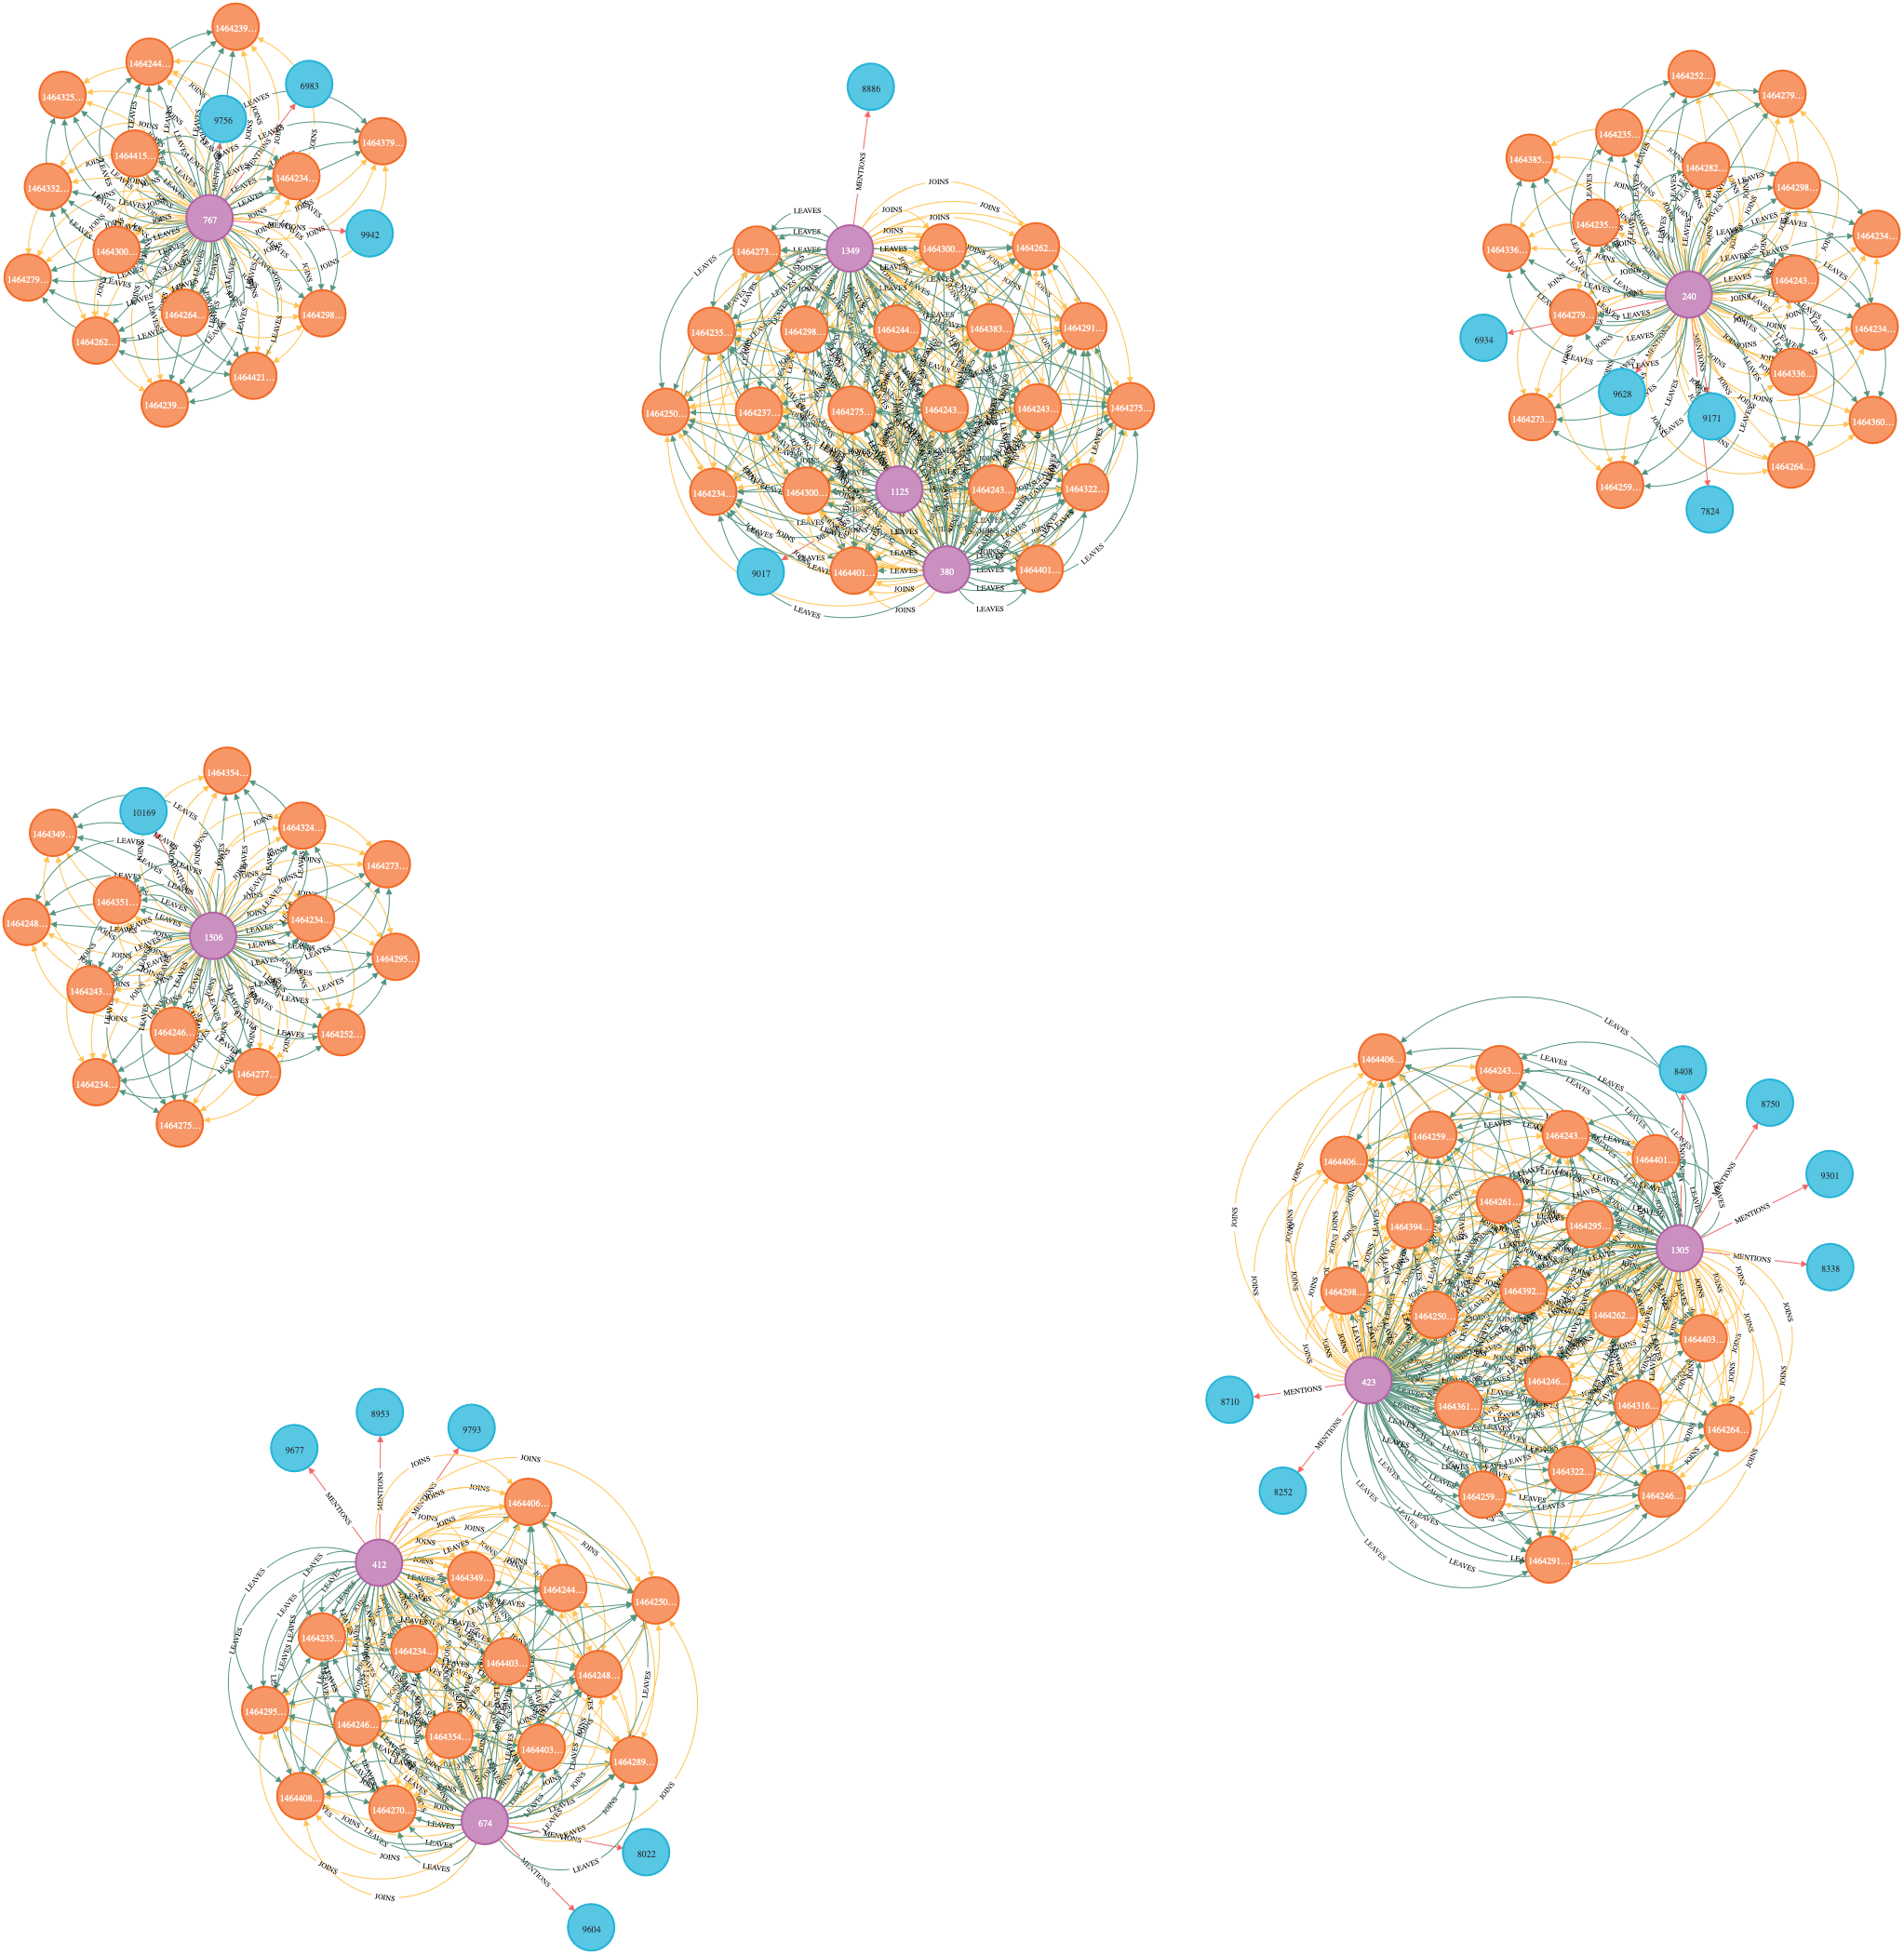
\includegraphics[scale=0.18]{img/Neo4j/graph0-filter.png}
    \centering
    \caption{Graph 1 filtered}
    \label{fig:Graph 1 filtered}
  \end{figure}
\end{landscape}

